\subsection{Entity-Relationship Schema}

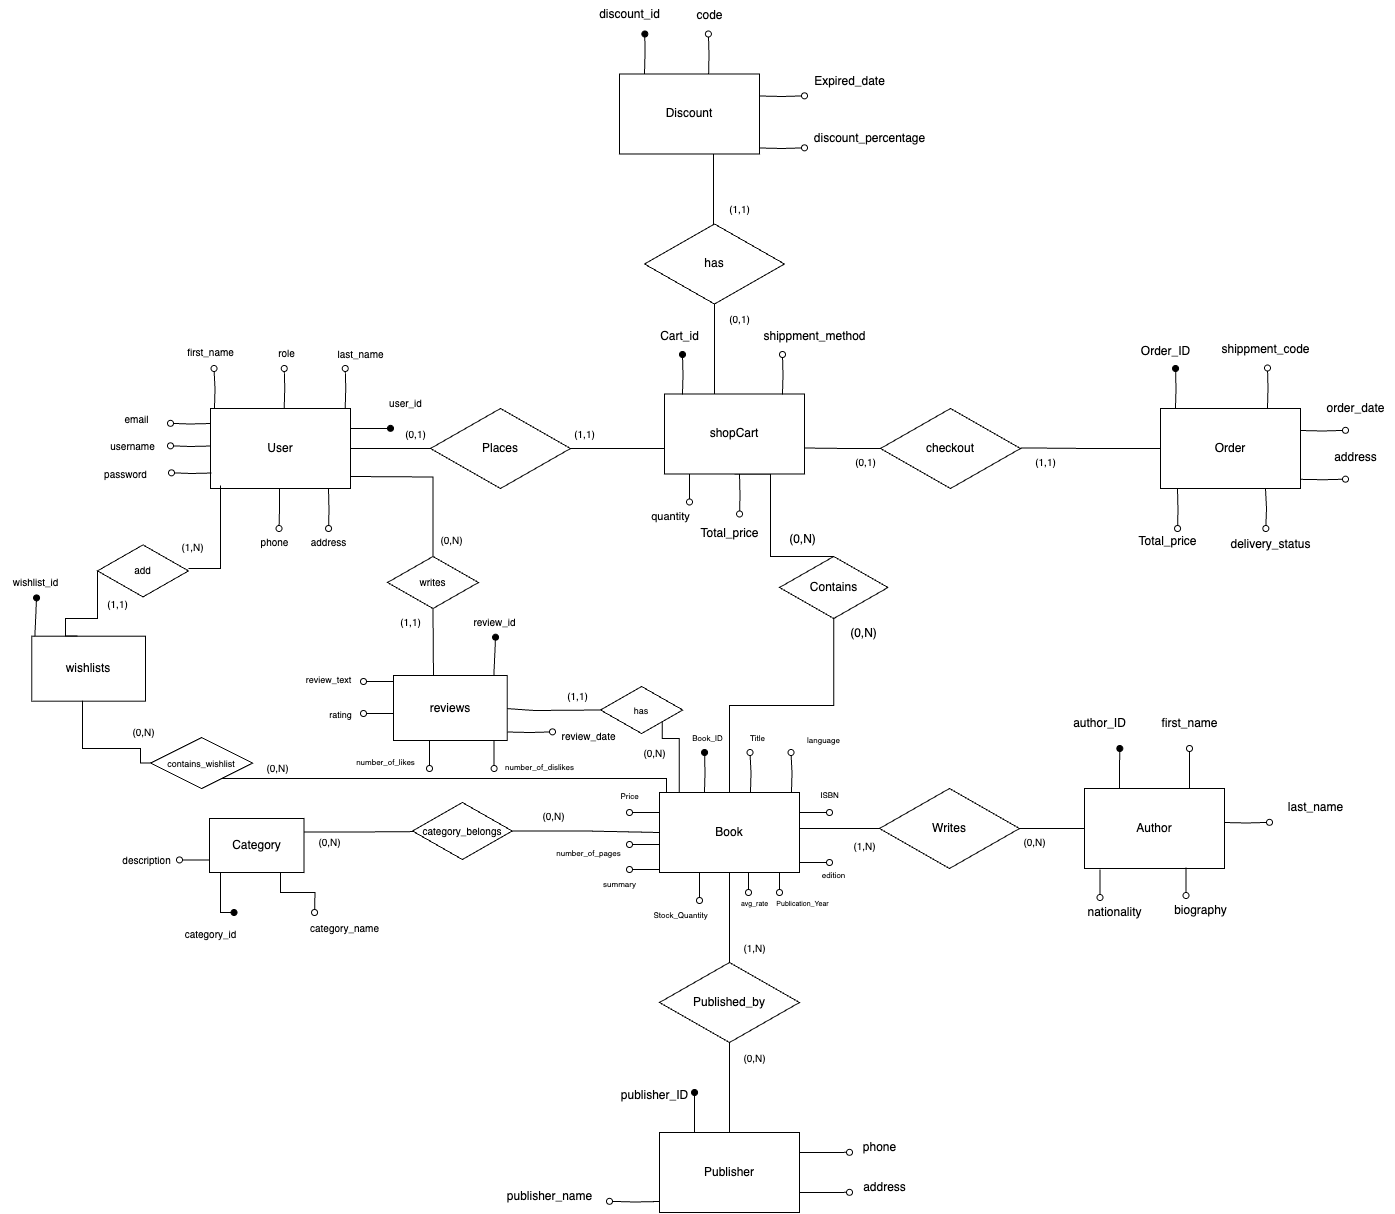
\includegraphics[width=0.8\linewidth]{wa-homework-template/photos/bookly.png}

\begin{figure}[h!]
    \centering
 
    \caption{ER-Diagram}
    \label{fig:enter-label}
\end{figure}\\


The ER schema contains the following entities:


\textbf{User} represents individuals who interact with the Bookly platform, such as browsing books, placing orders, writing reviews, and creating wishlists. Each user is uniquely identified by \texttt{user\_id} (type: SERIAL, primary key). The \texttt{username} (type: booklySchema.username\_domain, i.e., \texttt{VARCHAR(50)} with format constraints) must be unique, and the \texttt{password} (type: booklySchema.password\_domain, i.e., \texttt{VARCHAR(255)}) must have at least 8 characters. Users also have \texttt{first\_name} and \texttt{last\_name} (both of type: \texttt{VARCHAR(50)}), and a unique \texttt{email} (type: \texttt{VARCHAR(100)}). The optional \texttt{phone} field uses a custom domain (type: phone\_domain, i.e., \texttt{VARCHAR(20)}) that enforces a valid format, and \texttt{address} (type: \texttt{TEXT}) stores shipping or billing information. The \texttt{role} attribute is defined by an ENUM type \texttt{user\_role} (values: 'user', 'admin') and defaults to 'user'. Each user is associated with a unique shopping cart via the \texttt{shopcart} foreign key (type: INTEGER), linking to the \texttt{shopcart} entity (1–1 relationship).\\

\textbf{Author} captures metadata about individuals who have written books. Each author is identified by a unique \texttt{author\_id} (type: SERIAL, primary key). Other attributes include \texttt{first\_name} and \texttt{last\_name} (both of type: \texttt{VARCHAR(100)}), a \texttt{biography} field (type: TEXT) containing an optional description of the author's life or achievements, and \texttt{nationality} (type: \texttt{VARCHAR(100)}) describing the author’s country of origin. Authors can be linked to one or more books through the \texttt{writes} relationship, which is modeled as a many-to-many association.\\

\textbf{Publisher} represents companies or organizations that publish books. Each publisher has a unique \texttt{publisher\_id} (type: SERIAL, primary key), a \texttt{publisher\_name} (type: \texttt{VARCHAR(100)}), an optional \texttt{phone} number (type: \texttt{phone\_domain}), and an \texttt{address} (type: TEXT). Each book can be published by exactly one publisher, and this is modeled by the \texttt{published\_by} relationship (many-to-one).\\

\textbf{Category} is used to classify books by genre, theme, or other organizing criteria. It includes a \texttt{category\_id} (type: SERIAL, primary key), a \texttt{category\_name} (type: \texttt{VARCHAR(50)}), and an optional \texttt{description} (type: TEXT). A book can belong to one or more categories, managed by the \texttt{category\_belongs} relationship (many-to-many).\\

\textbf{Book} is the core item of the platform, representing all available reading material. Each book is uniquely identified by \texttt{book\_id} (type: SERIAL, primary key), and includes a \texttt{title} (type: \texttt{VARCHAR(150)}), optional \texttt{language} (type: \texttt{VARCHAR(50)}), and a unique \texttt{isbn} (type: \texttt{VARCHAR(20)}). The \texttt{price} (type: REAL) is a required field representing the cost. Additional attributes include \texttt{edition} (type: \texttt{VARCHAR(50)}), \texttt{publication\_year} (type: INTEGER) restricted between 1000 and the current year, \texttt{number\_of\_pages} (type: INTEGER, must be positive), and \texttt{stock\_quantity} (type: INTEGER, default 0, must be non-negative). The \texttt{average\_rate} (type: REAL) stores the average of user-submitted ratings, and \texttt{summary} (type: TEXT) provides an optional overview of the book. Books are connected to categories, publishers, authors, shopping carts, and reviews via appropriate relationships.\\


\textbf{ShopCart} represents a temporary list of books a user intends to purchase. Each cart has a \texttt{cart\_id} (type: SERIAL, primary key), a \texttt{shippment\_method} (type: ENUM \texttt{shippment\_method}, values: 'in\_person', 'credit\_card'), and a \texttt{user\_id} (type: INTEGER) as a unique foreign key referencing \texttt{users}, enforcing a 1–1 user-cart relationship. It also includes \texttt{created\_date} (type: TIMESTAMP, default: current time), \texttt{quantity} (type: INTEGER, default: 0), \texttt{discount} (type: INTEGER) as a foreign key referencing the \texttt{discounts} table, and \texttt{order} (type: INTEGER) as a foreign key referencing the \texttt{orders} table.\\

\textbf{Order} represents completed purchases. Each order has a unique \texttt{order\_id} (type: SERIAL, primary key), a \texttt{total\_amount} (type: NUMERIC(10,2)) representing the final price, a \texttt{payment\_method} (type: ENUM \texttt{payment\_method}), and a \texttt{payment\_date} (type: TIMESTAMP, default: current timestamp). Orders are linked to shopping carts (1–1), and may include discounts.\\

\textbf{Discount} defines promotional codes that reduce order totals. It includes a \texttt{discount\_id} (type: SERIAL, primary key), a unique \texttt{code} (type: \texttt{VARCHAR(50)}), a \texttt{discount\_percentage} (type: NUMERIC(5,2)) restricted to 0–100, and an optional \texttt{expired\_date} (type: DATE). Each discount can be associated with a shopping cart or order to adjust pricing.

\textbf{Reviews} captures feedback from users about books. Each review has a unique \texttt{review\_id} (type: SERIAL, primary key), and includes \texttt{user\_id} and \texttt{book\_id} (both of type: INTEGER) as foreign keys. It also includes \texttt{review\_text} (type: TEXT), a \texttt{rating} (type: INTEGER between 1 and 5), \texttt{review\_date} (type: TIMESTAMP, default: current timestamp), and optional counters for \texttt{number\_of\_likes} and \texttt{number\_of\_dislikes} (both of type: INTEGER). This entity supports the social and feedback features of the platform.